\subsection{Proxy}
Viene utilizzato per fornire un surrogato di un altro oggetto di cui si vuole controllare l’accesso. Questo surrogato deve quindi agire come l’oggetto che rappresenta e perciò devono condividere la stessa interfaccia.
Questo pattern ha diversi utilizzi pratici:
\begin{itemize}
\item \textbf{Remote proxy}: rappresentazione locale di un oggetto remoto (JavaRMI)
\item \textbf{Virtual proxy}: creazione ritardata di oggetti (Lazy instantiation)
\item \textbf{Protection proxy}: controllo degli accessi all’oggetto originale
\item \textbf{Puntatore intelligente}: per una gestione efficace della memoria (Copy on edit)
\end{itemize}
\begin{figure}[ht]
    \centering
    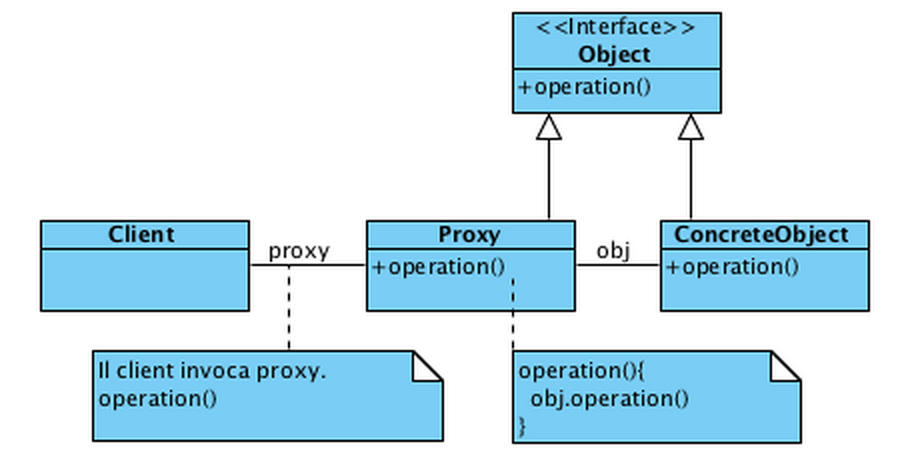
\includegraphics[width=0.8\textwidth]{immagini/proxy.png}
    \caption{Proxy}
\end{figure}
\FloatBarrier
